\documentclass[11pt]{article}
\usepackage[lmargin=1in,rmargin=1.75in,bmargin=1in,tmargin=1in]{geometry}

% For hyperlinking everything
\usepackage{hyperref}
\hypersetup{
	colorlinks=true, %set true if you want colored links
	linktoc=all,     %set to all if you want both sections and subsections linked
	linkcolor=blue,  %choose some color if you want links to stand out
}


\usepackage[latin1]{inputenc}
\usepackage{amsmath}
\usepackage{mathrsfs}  
\usepackage{amsfonts}
\usepackage{amssymb}
\usepackage{graphicx}
\usepackage{subfig}
\usepackage{caption}
\usepackage{algorithm}
%\usepackage{algcompatible}
%\usepackage{algorithmicx}
\usepackage{algpseudocode}

\usepackage{titlesec}
\titleformat{\section}{\fontfamily{lmss}\fontsize{14}{15}\bfseries}{\thesection}{1em}{}
\titleformat{\subsection}{\fontfamily{lmss}\fontsize{12}{15}\bfseries}{\thesubsection}{1em}{}




\usepackage{amsthm}

\newtheoremstyle{noit}
{10pt}% <Space above>
{10pt}% <Space below>
{}% <Body font>
{}% <Indent amount>
{\bfseries}% <Theorem head font>
{.}% <Punctuation after theorem head>
{.5em}% <Space after theorem headi>
{}% <Theorem head spec (can be left empty, meaning `normal')>

\newtheoremstyle{example}
{10pt}% <Space above>
{10pt}% <Space below>
{}% <Body font>
{20pt}% <Indent amount>
{\bfseries}% <Theorem head font>
{.}% <Punctuation after theorem head>
{.5em}% <Space after theorem headi>
{}% <Theorem head spec (can be left empty, meaning `normal')>


\newtheoremstyle{indented}{20pt}{20pt}{\addtolength{\leftskip}{2.5em}}{}{\bfseries}{.}{.5em}{}


\newtheorem{theorem}{Theorem}
\numberwithin{theorem}{section}
\newtheorem{lemma}[theorem]{Lemma}
\newtheorem{corollary}[theorem]{Corollary}
\newtheorem{observation}{Observation}
%\numberwithin{observation}{section}
%\numberwithin{definition}{section}
\newtheorem{conjecture}{Conjecture}
\newtheorem{Qu}{Question}
\newcommand{\QU}{\begin{Qu}\normalfont}

\theoremstyle{noit}
\newtheorem{fact}{Fact}
\newtheorem{definition}{Definition}

\theoremstyle{indented}
\newtheorem{example}{Example}

\theoremstyle{indented}
\newtheorem{problem}{Problem}


%\newenvironment{proof}{\noindent{\bf Proof:} \hspace*{1em}}{
%    \hspace*{\fill} $\Box$ }
%\newenvironment{proof_of}[1]{\noindent {\bf Proof of #1:}
%    \hspace*{1em} }{\hspace*{\fill} $\Box$ }
%\newenvironment{proof_claim}{\begin{quotation} \noindent}{
%    \hspace*{\fill} $\diamond$ \end{quotation}}
\newcommand{\vs}[1]{\vspace{#1}}

\newcommand{\lecture}[2]{
 \noindent
\begin{center}
	\framebox{
		\vbox{
			\hbox to 5.78in { {\bf CSCE 411: Design and Analysis of Algorithms (Honors)} \hfill  }
			\vspace{2mm}
			\hbox to 5.78in { {\Large \hfill Lecture #1\hfill} }
			\vspace{2mm}
			\hbox to 5.78in { {\it Date: #2 \hfill Samson Zhou} }
		}
	}
\end{center}
\vspace*{4mm}
}

\newcommand{\week}[2]{
 \noindent
\begin{center}
	\framebox{
		\vbox{
			\hbox to 5.78in { {\bf CSCE 411: Design and Analysis of Algorithms (Honors)} \hfill  }
			\vspace{2mm}
			\hbox to 5.78in { {\Large \hfill Week #1\hfill} }
			\vspace{2mm}
			\hbox to 5.78in { {\it Date: #2 \hfill Nate Veldt, updated by Samson Zhou} }
		}
	}
\end{center}
\vspace*{4mm}
}

\newcommand{\sweek}[2]{
 \noindent
\begin{center}
	\framebox{
		\vbox{
			\hbox to 5.78in { {\bf CSCE 411: Design and Analysis of Algorithms (Honors)} \hfill  }
			\vspace{2mm}
			\hbox to 5.78in { {\Large \hfill Week #1\hfill} }
			\vspace{2mm}
			\hbox to 5.78in { {\it Date: #2 \hfill Samson Zhou} }
		}
	}
\end{center}
\vspace*{4mm}
}

\newcommand{\hw}[2]{
	\noindent
	\begin{center}
		\framebox{
			\vbox{
				\hbox to 5.78in { {\bf CSCE 411: Design and Analysis of Algorithms} \hfill  }
				\vspace{2mm}
				\hbox to 5.78in { {\Large \hfill Homework #1\hfill} }
				\vspace{2mm}
				\hbox to 5.78in { {\it Due date: #2 \hfil} }
			}
		}
	\end{center}
	\vspace*{4mm}
}



\newcommand{\under}[1]{\underline{\hspace{#1}}}
\setlength{\parindent}{0em}

%\usepackage[tagged]{accessibility}

% Graph terms
\newcommand{\vol}{\textbf{vol}}
\newcommand{\cut}{\textbf{cut}}


% Matrices
\newcommand{\mA}{\textbf{A}}
\newcommand{\mB}{\textbf{B}}

% vectors
\newcommand{\ve}{\textbf{e}}
\newcommand{\vx}{\textbf{x}}


% Other
\newcommand{\calN}{\mathcal{N}}

\usepackage{mathtools}
\DeclarePairedDelimiter\ceil{\lceil}{\rceil}
\DeclarePairedDelimiter\floor{\lfloor}{\rfloor}


\newcommand*{\aitem}{ \item[{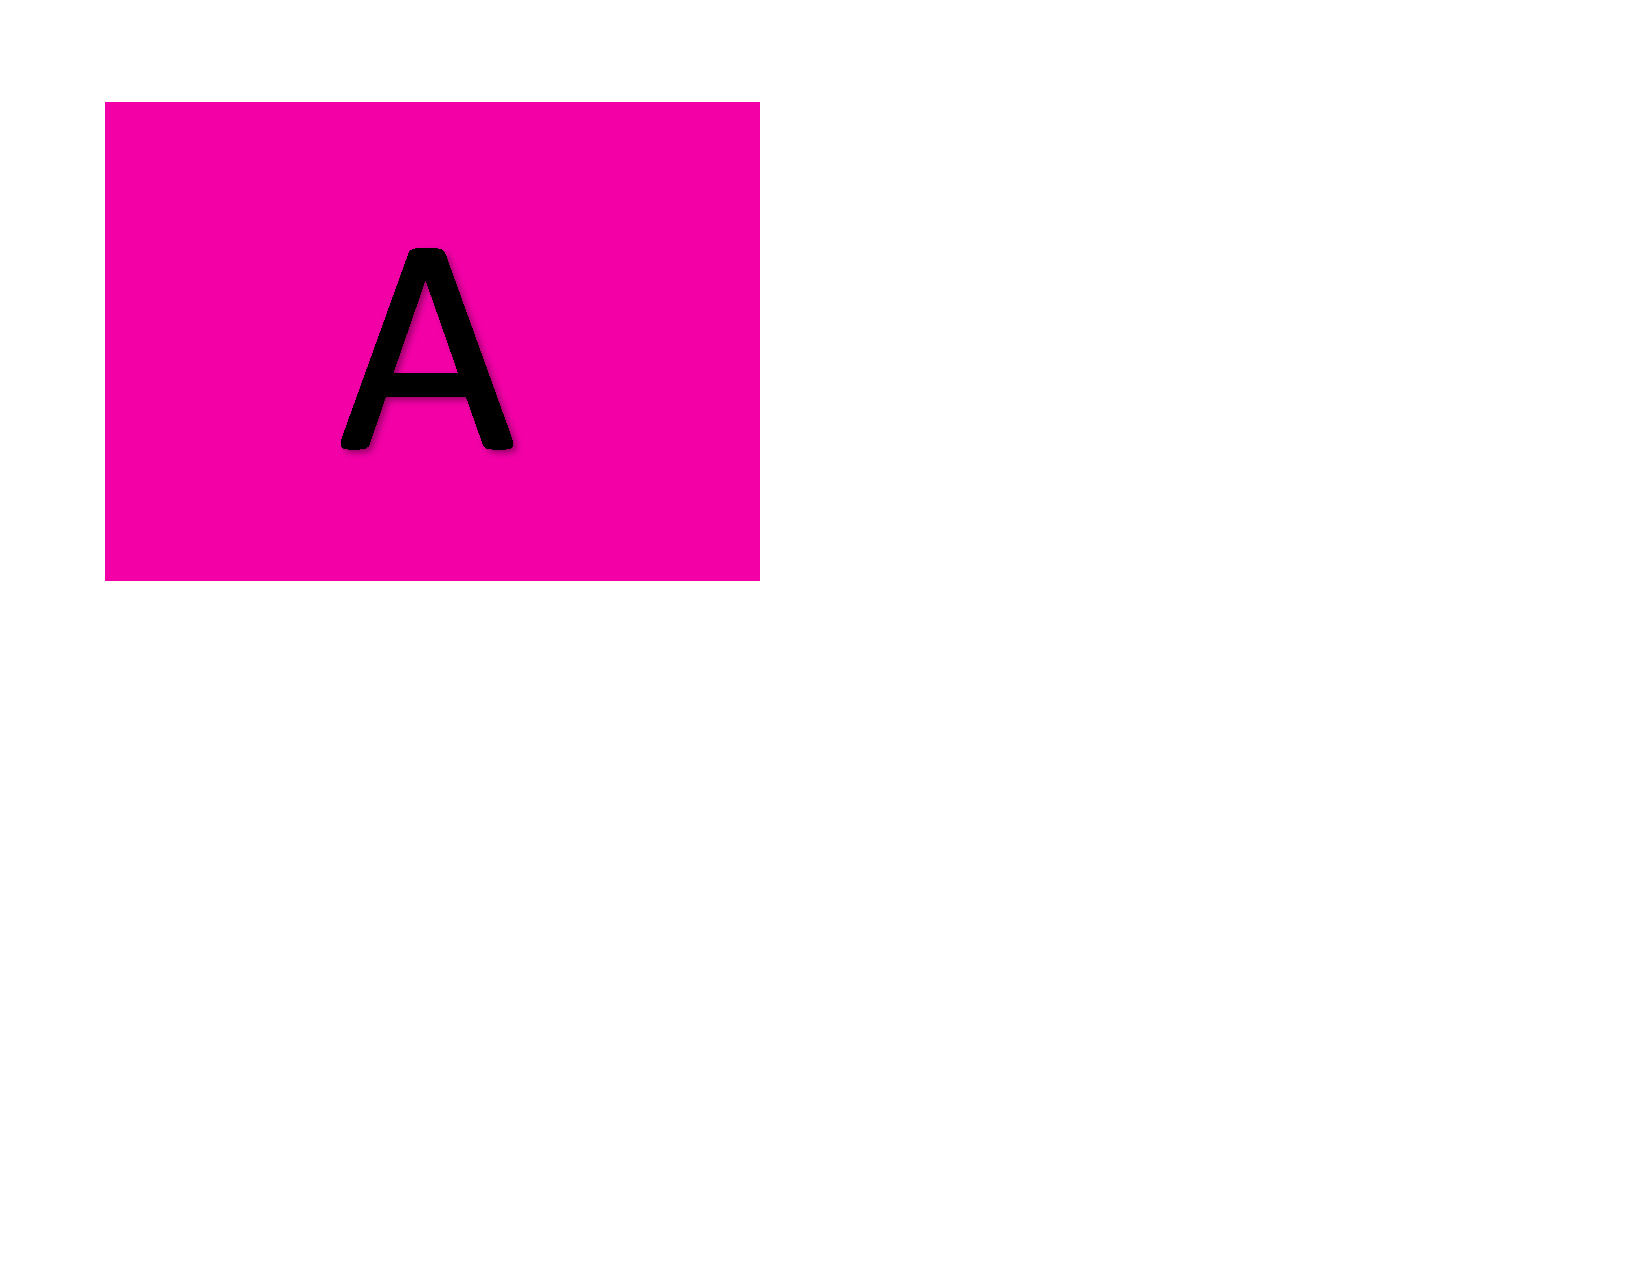
\includegraphics[width=0.8cm,height=0.5cm]{figures/A}} ]  }
\newcommand*{\bitem}{ \item[{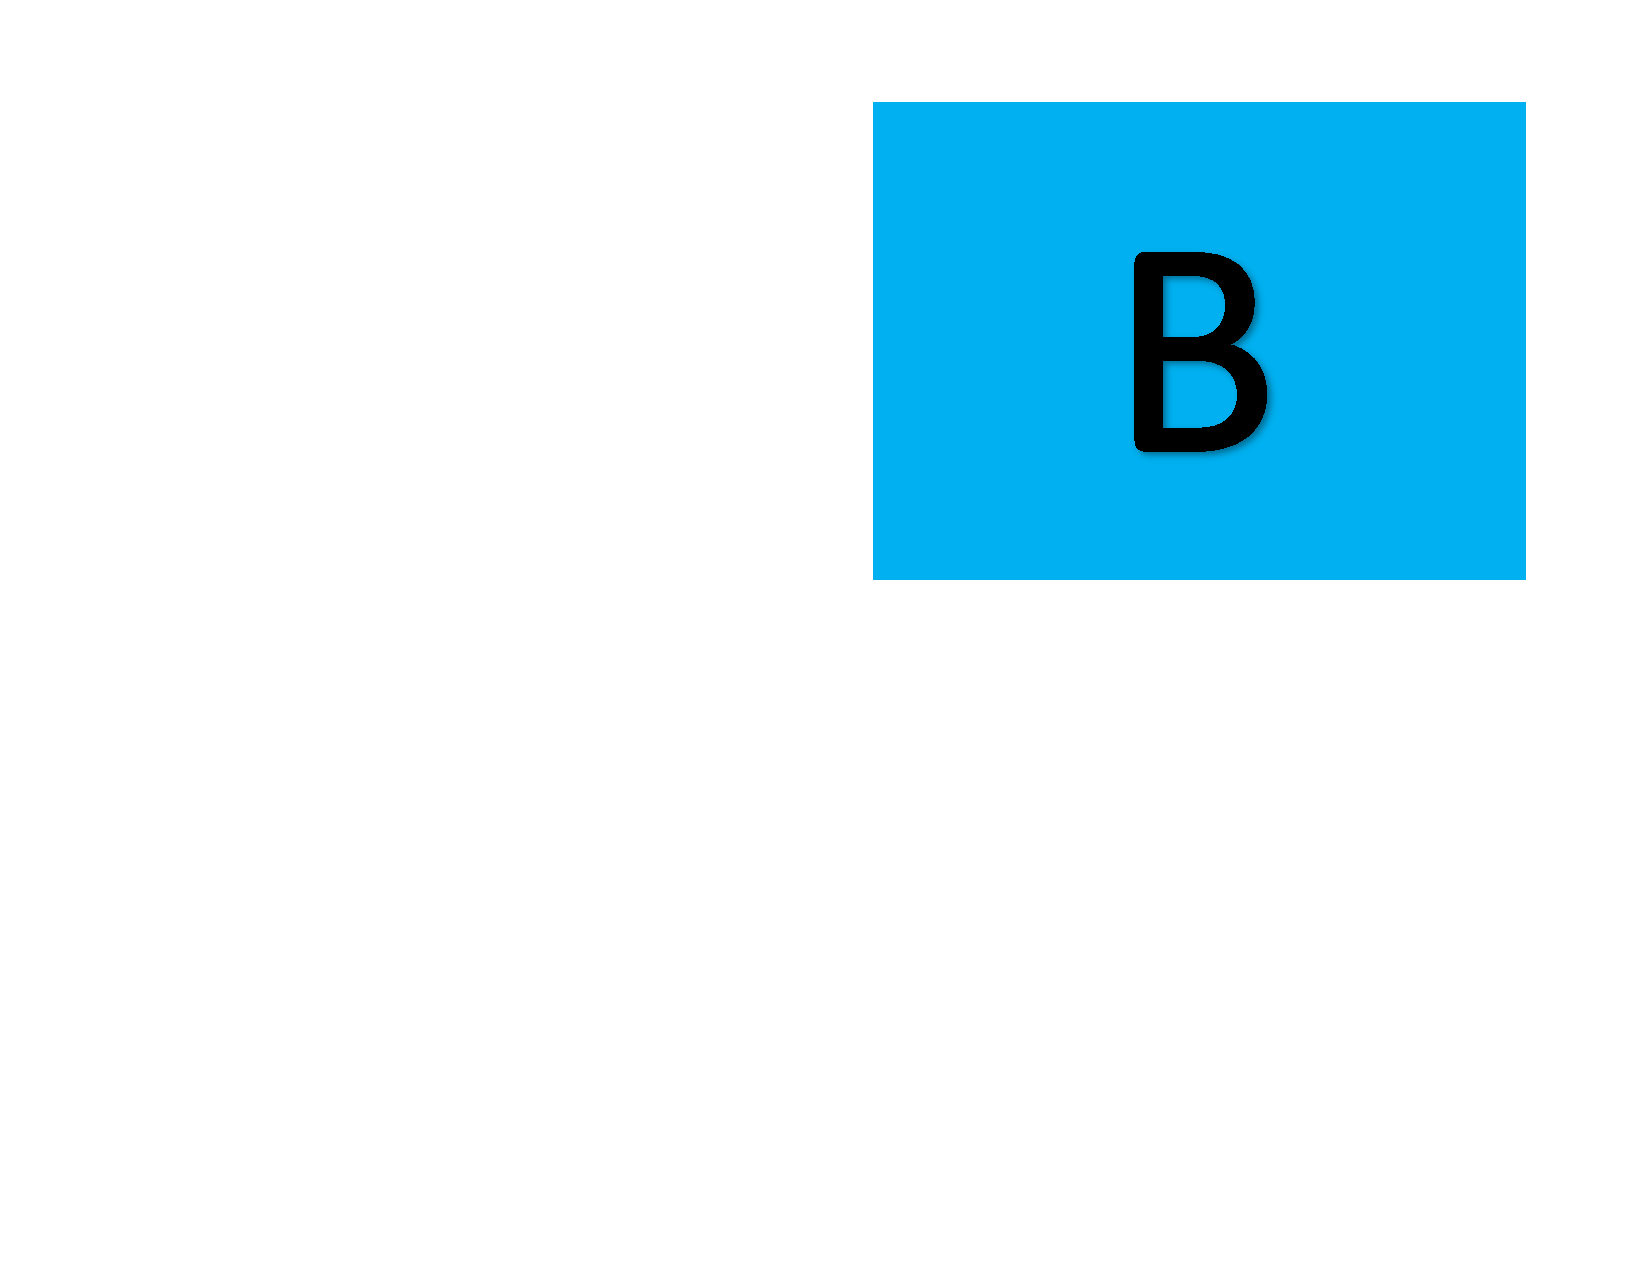
\includegraphics[width=0.8cm,height=0.5cm]{figures/B}} ]  }
\newcommand*{\citem}{ \item[{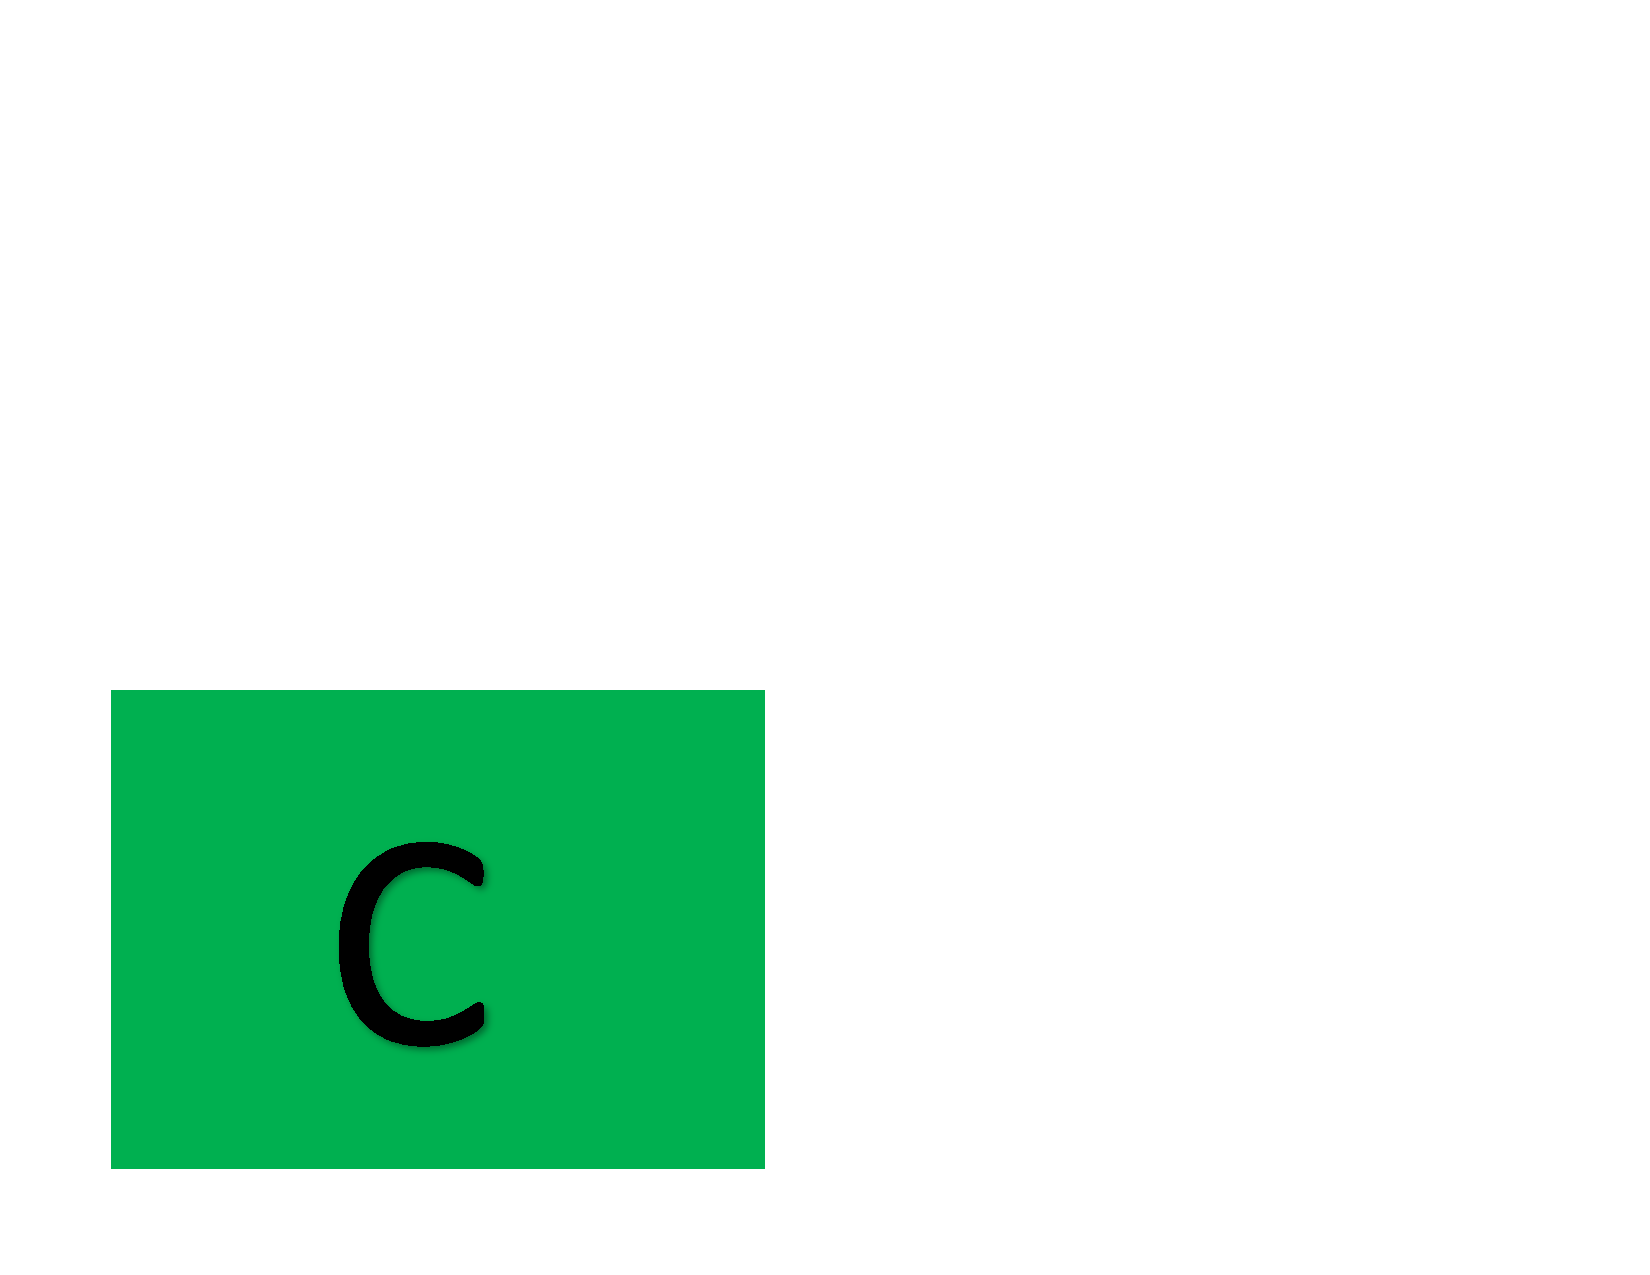
\includegraphics[width=0.8cm,height=0.5cm]{figures/C}} ]  }
\newcommand*{\ditem}{ \item[{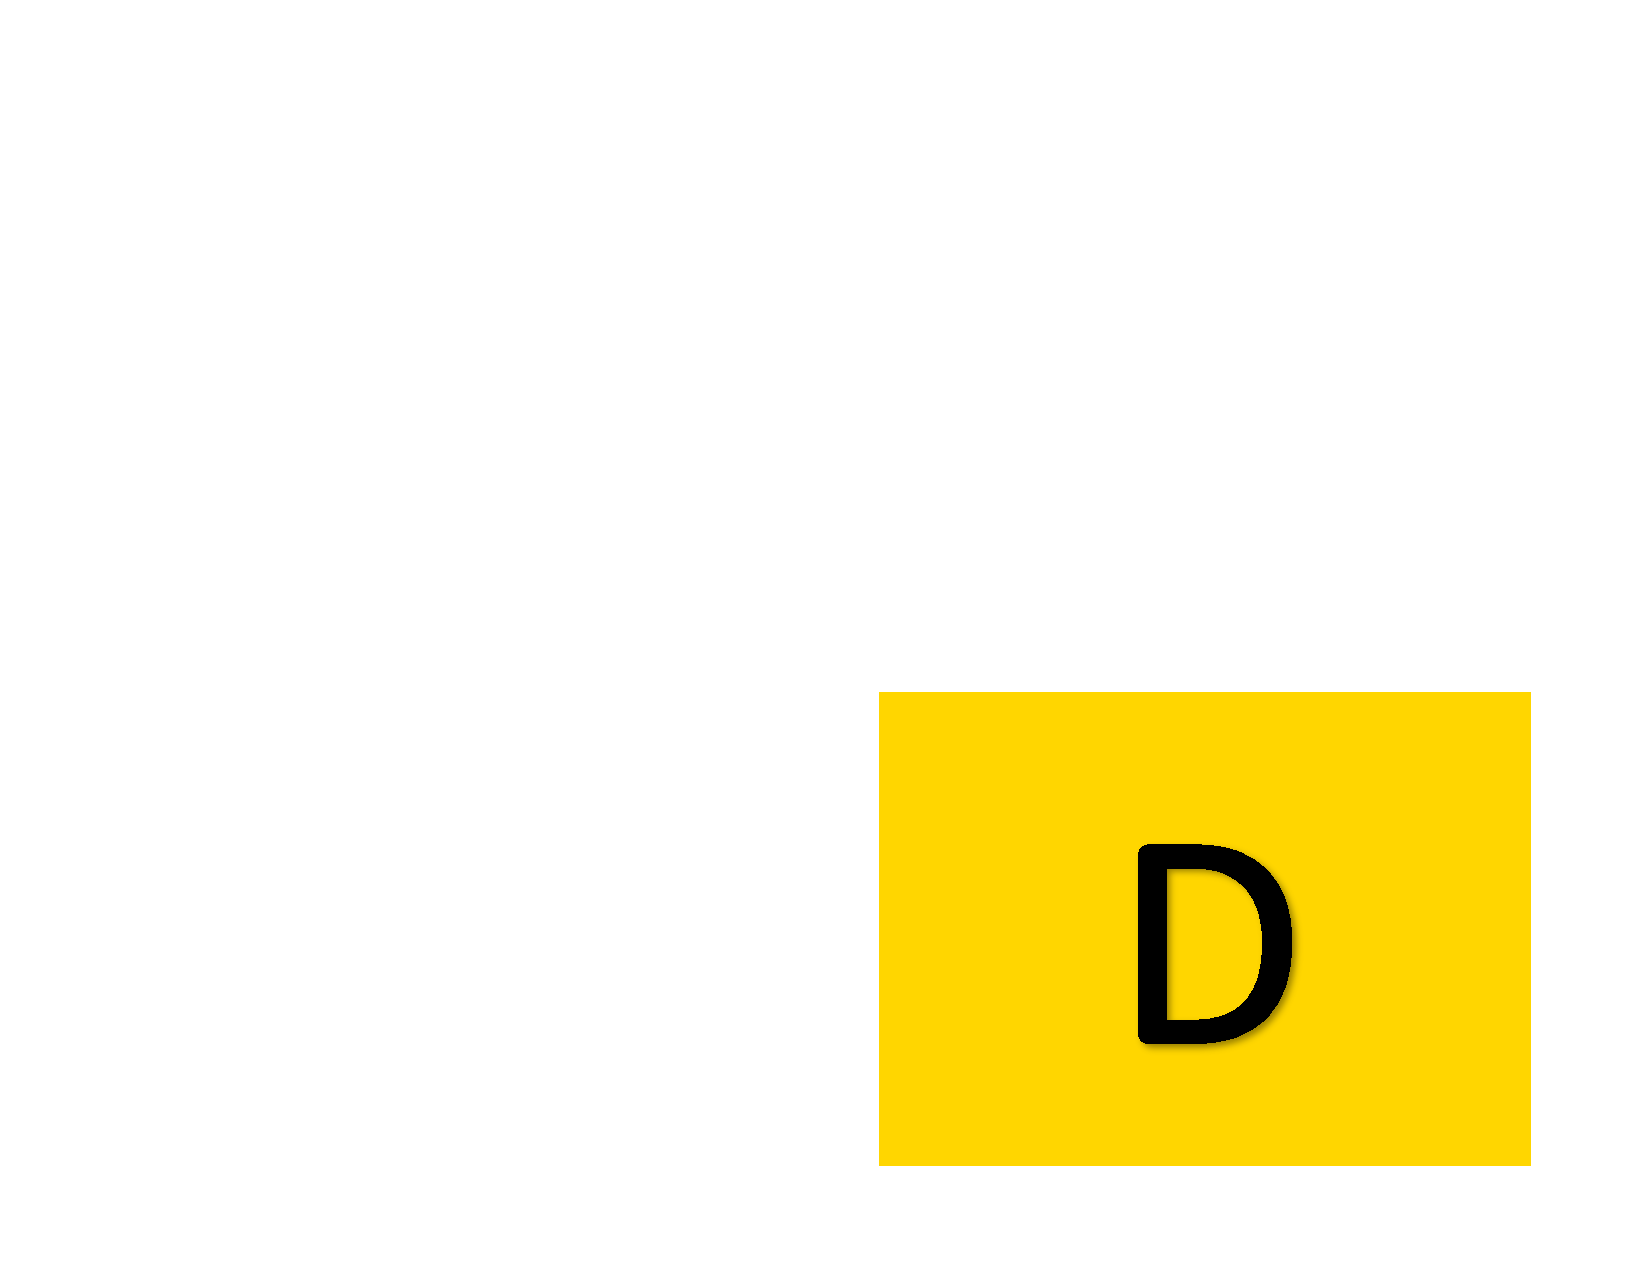
\includegraphics[width=0.8cm,height=0.5cm]{figures/D}} ]  }
\newcommand*{\eitem}{ \item[{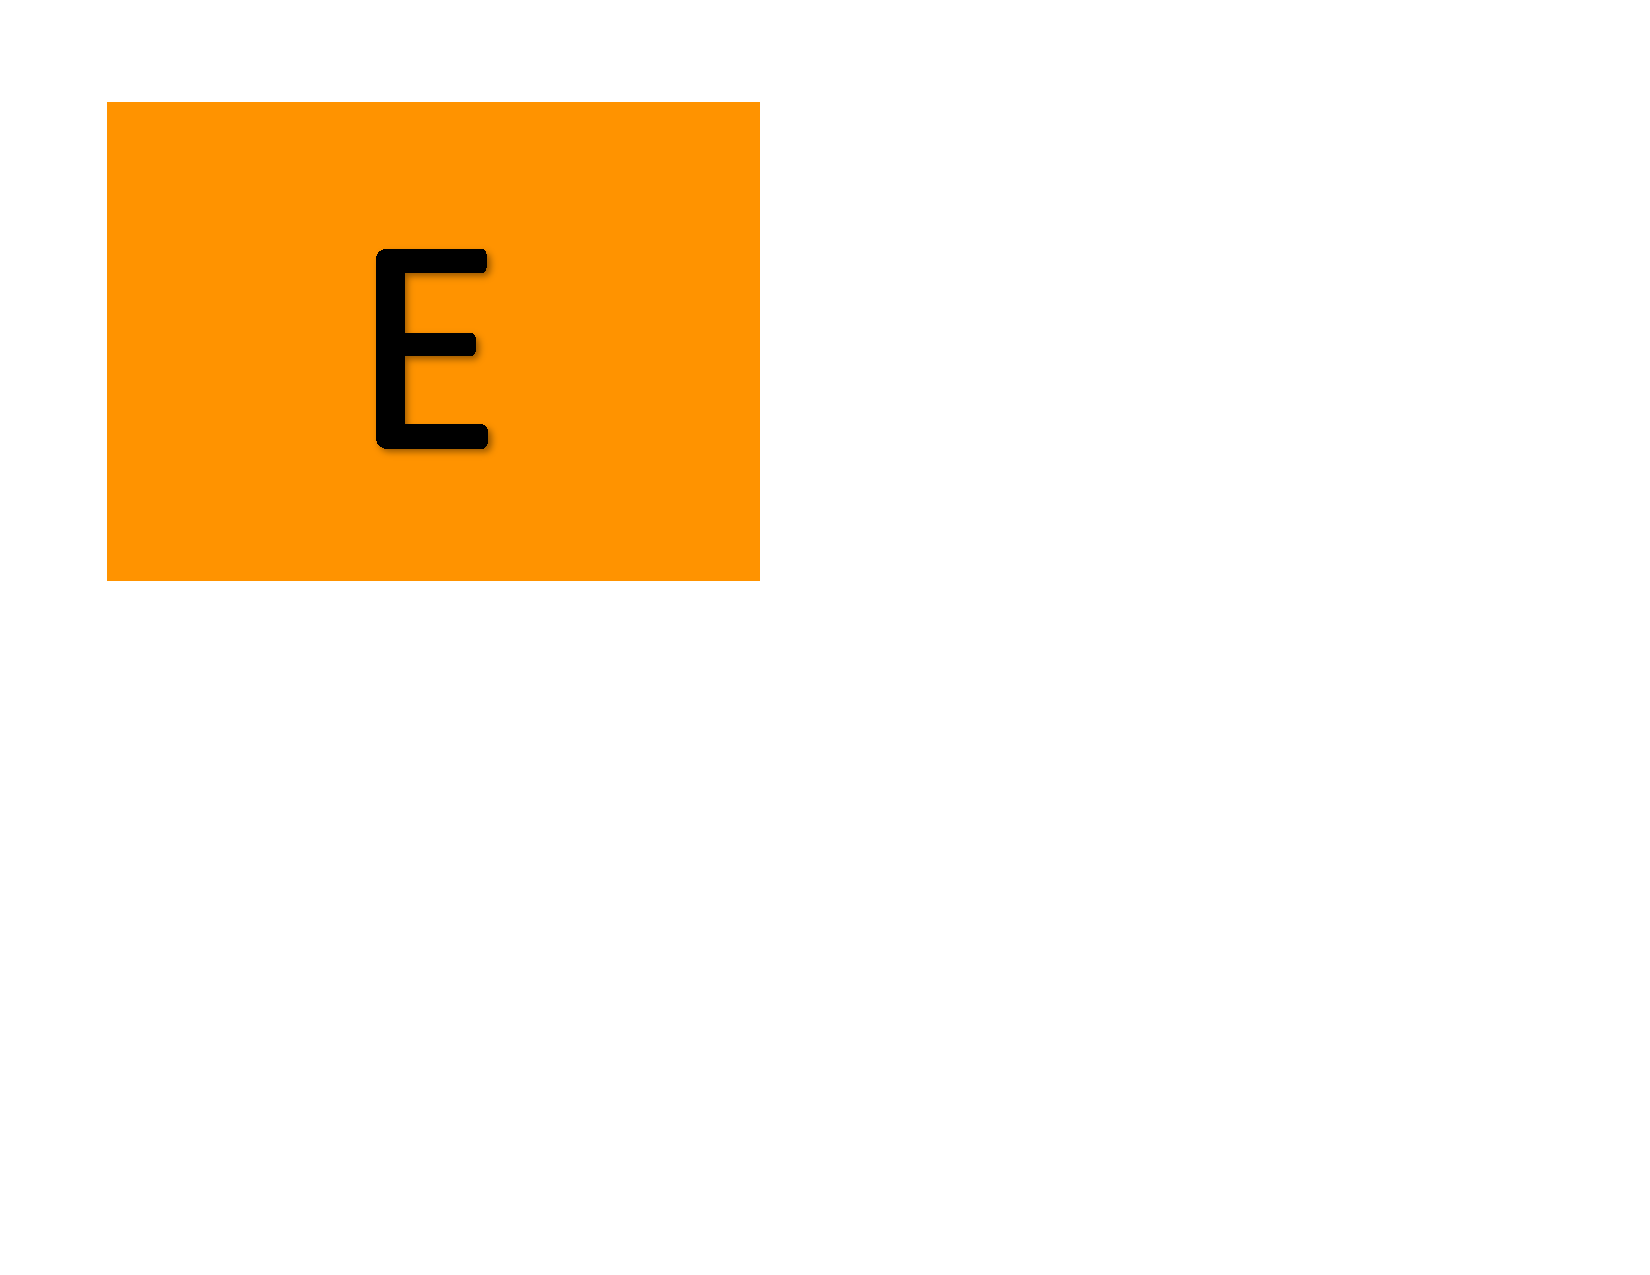
\includegraphics[width=0.8cm,height=0.5cm]{figures/E}} ]  }
\newcommand*{\fitem}{ \item[{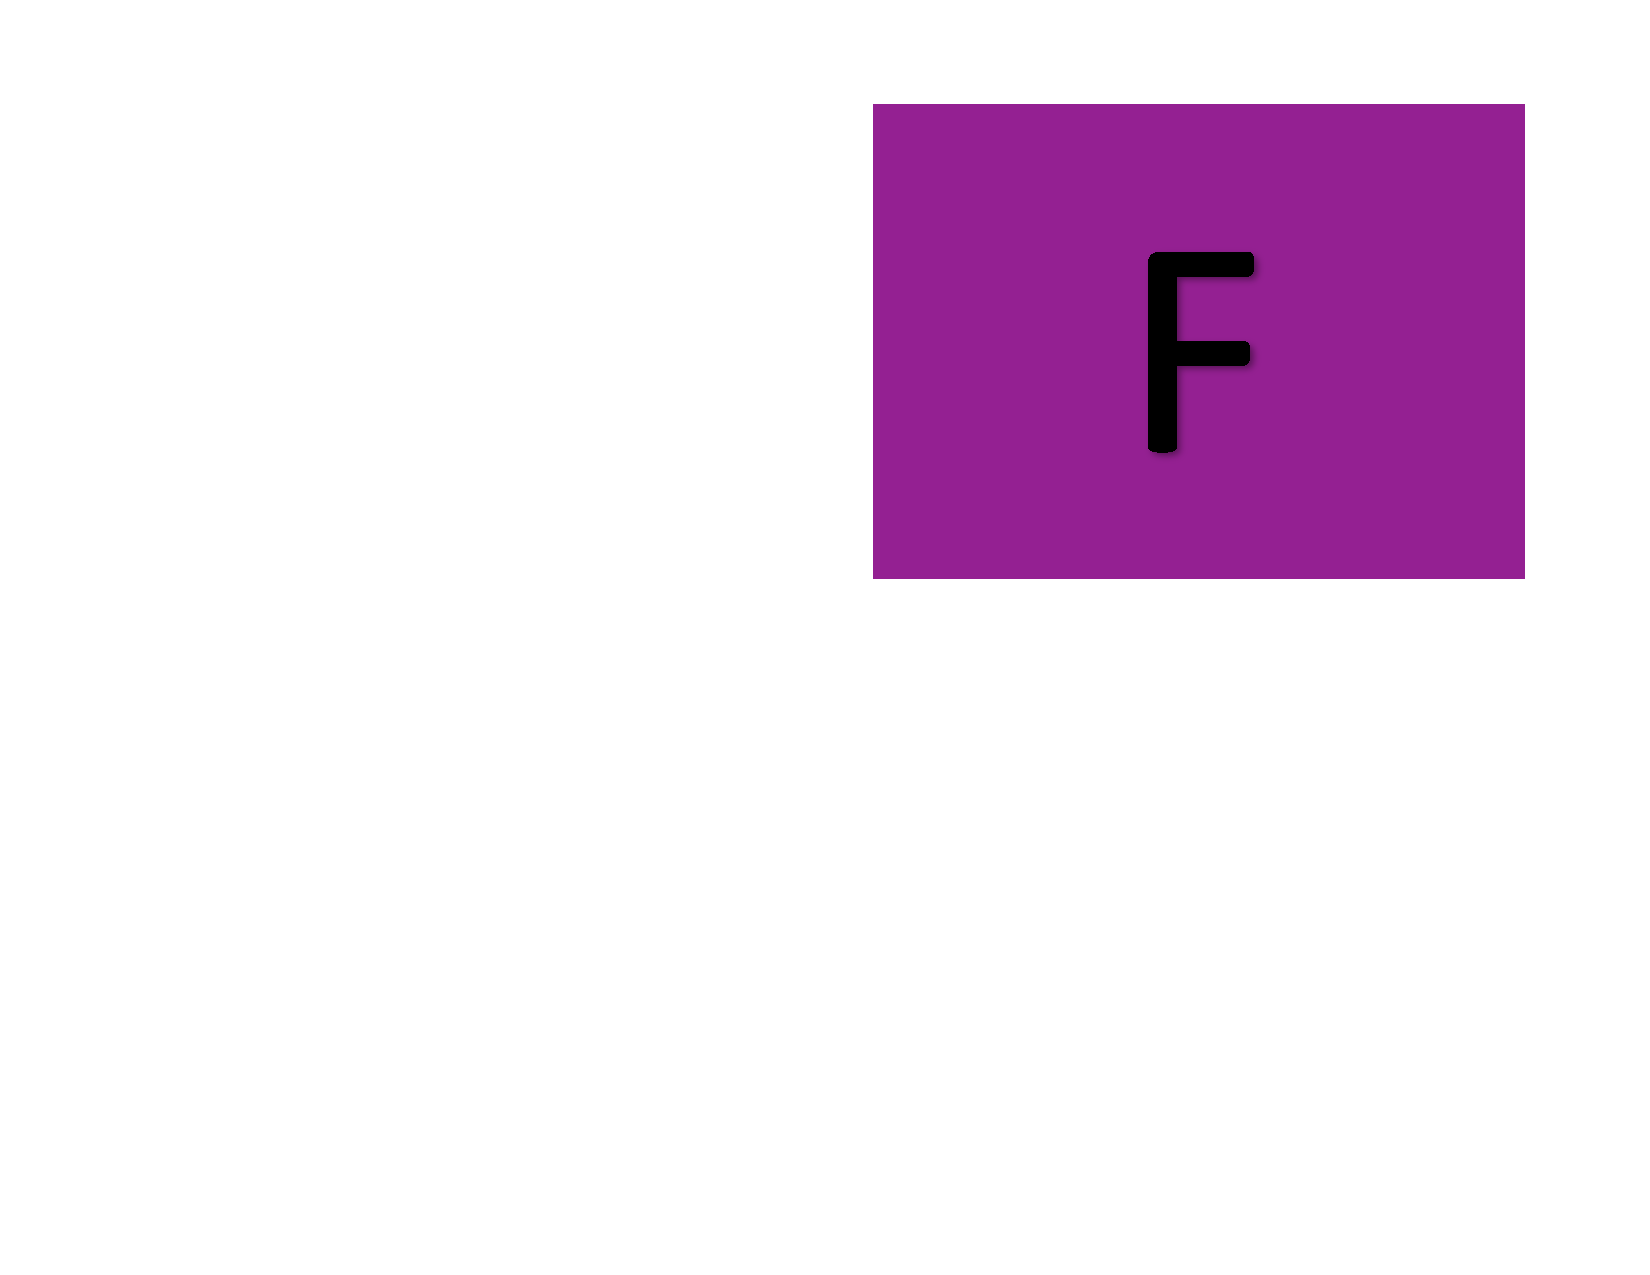
\includegraphics[width=0.8cm,height=0.5cm]{figures/F}} ]  }


\newcommand{\hide}[1]{\underline{\phantom{#1 #1}}}

\usepackage{setspace}

\onehalfspacing
\usepackage{tikz}
\usetikzlibrary{arrows.meta,positioning,calc}

\begin{document}
% Fill in the date when scheduling this lecture.
\sweek{12a: Hashing}{November 10}

% Suggested 120-minute schedule, including a five-minute break:
% 0--10: dictionaries, hashing, and randomized algorithms.
% 10--20: collisions and the birthday effect.
% 20--40: chaining and the definition of universal hashing.
% 40--55: expected search time and discussion.
% 55--60: break.
% 60--75: open addressing, deletion, and double hashing.
% 75--85: resizing and amortized analysis.
% 85--100: fingerprints and rolling hashes.
% 100--112: Karp--Rabin and its collision guarantee.
% 112--120: verification and review questions.
% The two optional extensions are outside this schedule.

\section{Dictionaries and Hashing}
A dictionary stores keys and their associated values. A compiler might store
the type of each variable, while a website might store the account associated
with each username.

We want to support three operations:
\begin{itemize}
    \item \textsc{Insert}$(x,v)$: store or update the value associated with $x$.
    \item \textsc{Search}$(x)$: return its value, or report that $x$ is absent.
    \item \textsc{Delete}$(x)$: remove $x$ if it is present.
\end{itemize}

\paragraph{Why not use an array?}
Suppose the keys are integers from $0$ to $10^{12}$, but only one million keys
are present. What is the disadvantage of using the key itself as an array index?
\vs{1cm}
% Answer: The array requires space for the whole universe, even though almost
% all of its entries are unused.

A \emph{hash function} maps a large universe into a smaller set of buckets:
\begin{equation*}
    h:U\longrightarrow\{0,1,\ldots,B-1\}.
\end{equation*}
We use $h(x)$ to decide where to store the key $x$.

\begin{Qu}
    If $x\neq y$ but $h(x)=h(y)$, which conclusion must follow?
    \begin{itemize}
        \aitem The dictionary gives an incorrect answer
        \bitem The dictionary must have a way to distinguish $x$ from $y$
        \citem No dictionary can store both keys
    \end{itemize}
\end{Qu}
% Answer: (b). Store the actual keys and compare them when searching.

\vfill
For our dictionary bounds, assume that keys occupy $O(1)$ machine words,
key comparison takes $O(1)$ time, and evaluating $h$ takes $O(1)$ time.
We will account separately for the cost of processing long strings.

\newpage
\subsection*{Where does randomness enter?}
Instead of using one fixed hash function for every input, we can choose a
function randomly when building the table. The resulting dictionary still
compares actual keys before returning an answer.

\paragraph{Monte Carlo algorithms}
A Monte Carlo algorithm has a prescribed running-time bound, but may return
\hide{an incorrect answer.} For each fixed input $x$, we want
\begin{equation*}
    \Pr[A(x)\neq f(x)]\leq\delta.
\end{equation*}
The probability is over the random choices of the algorithm.

\paragraph{Las Vegas algorithms}
A Las Vegas algorithm always returns the correct answer, but its running time
is \hide{a random variable.} We usually bound its expected running time.
Randomized quicksort is one example.

\begin{Qu}
    A hash-table implementation compares full keys, but randomly chooses its
    hash function. What can a collision change?
    \begin{itemize}
        \aitem Whether the answer is correct
        \bitem How much work an operation performs
        \citem Both the answer and its correctness guarantee
    \end{itemize}
\end{Qu}
% Answer: (b). The dictionary remains exact; randomness affects its cost.

\paragraph{Reducing the probability of error}
Suppose a decision algorithm errs with probability at most $1/3$. Run it an
odd number $k$ of times independently and take a majority vote. Its error
probability becomes $e^{-\Omega(k)}$.

If an equality test only makes false-positive errors, each with probability
at most $\delta$, we can instead accept only when all $k$ independent runs
accept. The new error bound is \hide{\ensuremath{\delta^k}}.

\vfill
Why is it important to use fresh randomness in the repeated runs?
\vs{.7cm}
% Answer: Reusing exactly the same random choices can reproduce exactly the
% same mistake. It does not give the independence needed for amplification.

\newpage
\section{Collisions}
A \emph{collision} is a pair of distinct keys $x,y$ with $h(x)=h(y)$.
If $|U|>B$, can we choose a function with no collisions at all?
\vs{.7cm}
% Answer: No, by the pigeonhole principle.

\paragraph{Counting colliding pairs}
Fix distinct keys $x_1,\ldots,x_n$. For now, imagine that each key independently
chooses a uniformly random bucket. Let $I_{ij}$ be 1 if $x_i$ and $x_j$ collide,
and 0 otherwise. Then
\begin{equation*}
    C=\sum_{i<j}I_{ij}
\end{equation*}
counts the number of colliding pairs.

For a fixed pair, $\mathbb E[I_{ij}]=\hide{1/B}$. Therefore,
\begin{equation*}
    \mathbb E[C]=\sum_{i<j}\mathbb E[I_{ij}]
        =\hide{\binom n2\frac1B}.
\end{equation*}

\paragraph{The birthday effect}
Under this independent uniform model, for $n\leq B$,
\begin{equation*}
    \Pr[\text{no collision}]
      =\prod_{i=0}^{n-1}\left(1-\frac{i}{B}\right)
      \approx e^{-n(n-1)/(2B)}.
\end{equation*}
This approximation is accurate when $n=O(\sqrt B)$ and $B$ is large.
Thus collisions become likely around $n=\hide{\sqrt B}$, even though
most buckets are still empty.

\begin{Qu}
    If $n=1000$ and $B=10^6$, approximately how many colliding pairs do we
    expect? Does a collision somewhere make every search slow?
\end{Qu}
\vs{1cm}
% Answer: The expectation is 0.4995. Under the ideal model, the probability
% of at least one collision is about 1-exp(-0.4995), or 0.393. A search only
% examines the keys relevant to its own bucket.

\newpage
\subsection*{Resolving collisions by chaining}
Each bucket stores a list of the keys that hash to it. To search for $x$, scan
bucket $h(x)$ and compare $x$ against the stored \hide{keys.}

\paragraph{Example}
Let $B=7$, let $h(x)=x\bmod 7$, and insert
\begin{equation*}
    10,\ 17,\ 24,\ 8,\ 15,\ 9.
\end{equation*}
The table below displays each chain in insertion order.

\begin{center}
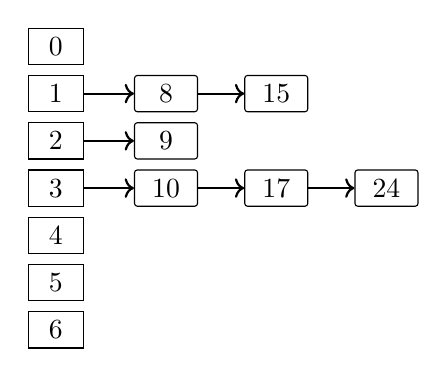
\begin{tikzpicture}[x=1cm,y=0.6cm,
    bucket/.style={draw,minimum width=0.7cm,minimum height=0.45cm},
    key/.style={draw,rounded corners=1pt,minimum width=0.8cm,minimum height=0.45cm},
    link/.style={->,thick}]
    \foreach \i in {0,...,6} {\node[bucket] (b\i) at (0,-\i) {\i};}
    \node[key] (k8) at (1.4,-1) {8};
    \node[key] (k15) at (2.8,-1) {15};
    \draw[link] (b1)--(k8); \draw[link] (k8)--(k15);
    \node[key] (k9) at (1.4,-2) {9}; \draw[link] (b2)--(k9);
    \node[key] (k10) at (1.4,-3) {10};
    \node[key] (k17) at (2.8,-3) {17};
    \node[key] (k24) at (4.2,-3) {24};
    \draw[link] (b3)--(k10); \draw[link] (k10)--(k17); \draw[link] (k17)--(k24);
\end{tikzpicture}
\end{center}

\begin{Qu}
    How many stored keys does each search compare?
    \begin{itemize}
        \aitem \textsc{Search}$(24)$: \hide{3}
        \bitem \textsc{Search}$(31)$: \hide{3}
        \citem \textsc{Search}$(9)$: \hide{1}
    \end{itemize}
\end{Qu}

\paragraph{Deleting a key}
How would the table change after \textsc{Delete}$(17)$?
\vs{.7cm}
% Answer: Remove 17 from bucket 3 and reconnect the link from 10 to 24.

\vfill
The \emph{load factor} is $\alpha=n/B$, the average number of keys per bucket.
Chaining allows $\alpha>1$, but longer chains mean more work.

\newpage
\section{Universal Hashing}
The function $h(x)=x\bmod B$ sends every multiple of $B$ to
\hide{bucket zero.} Could a different deterministic function avoid all bad
sets of keys?

\begin{theorem}
    If $|U|>(n-1)B$, every function from $U$ to $B$ buckets has $n$ distinct
    keys that all hash to the same bucket.
\end{theorem}

\paragraph{Finding a bad set}
Some bucket has at least
\begin{equation*}
    \left\lceil\frac{|U|}{B}\right\rceil\geq\hide{n}
\end{equation*}
preimages. Which principle gives this conclusion?
\vs{.5cm}
% Answer: The pigeonhole principle.

Choose $n$ of these keys. A search through their chain can require
\hide{\ensuremath{\Theta(n)}} comparisons.

\paragraph{Choosing a function at random}
A family $\mathcal H$ is \emph{universal} if, for every distinct $x,y\in U$,
a uniformly random $h\in\mathcal H$ satisfies
\begin{equation*}
    \Pr_h[h(x)=h(y)]\leq\frac1B.
\end{equation*}
We choose one function and use it throughout the table.

\begin{Qu}
    Which statement does universality guarantee?
    \begin{itemize}
        \aitem Every bucket gets exactly $n/B$ keys
        \bitem There are no collisions with high probability
        \citem Each fixed pair collides with probability at most $1/B$
    \end{itemize}
\end{Qu}
% Answer: (c). Universality is a bound for each fixed pair, not a guarantee
% that the entire table is collision-free or perfectly balanced.

\vfill
\textbf{To be clear.} The keys and queries in our analysis are fixed
independently of the sampled function. Choosing keys after seeing the function
need not satisfy the same guarantee.

\newpage
\subsection*{Bounding the expected search time}
\begin{lemma}
    With universal hashing and separate chaining, a fixed search has expected
    running time $O(1+\alpha)$, where $\alpha=n/B$.
\end{lemma}

\paragraph{First, consider an unsuccessful search}
Let $S$ be the fixed set of $n$ stored keys and let $x\notin S$ be the query.
The number of stored keys in its bucket is
\begin{equation*}
    C_x=\sum_{y\in S}\mathbf 1[h(y)=h(x)].
\end{equation*}
By linearity of expectation,
\begin{equation*}
    \mathbb E[C_x]
      =\sum_{y\in S}\Pr[h(y)=h(x)]
      \leq\sum_{y\in S}\hide{\frac1B}
      =\hide{\frac nB}.
\end{equation*}
Hashing the key costs $O(1)$, and scanning the chain costs $O(C_x)$. Thus,
the expected total is \hide{\ensuremath{O(1+n/B)}}.

\paragraph{Next, consider a successful search}
If $x\in S$, its chain contains $x$ itself plus the other keys colliding with
$x$. The expected chain length is at most
\begin{equation*}
    \hide{1+\frac{n-1}{B}}.
\end{equation*}
This gives the same asymptotic upper bound.

\begin{Qu}
    Which step required independence between different collision events?
    \begin{itemize}
        \aitem Linearity of expectation
        \bitem Applying the collision bound to each pair
        \citem Neither step
    \end{itemize}
\end{Qu}
% Answer: (c). Linearity of expectation holds for dependent variables too.

\paragraph{Return to the birthday effect}
With one million keys and one million buckets, there may be many collisions
in the whole table. Why can a fixed search still have expected $O(1)$ cost?
\vs{.7cm}
% Answer: Counting all colliding pairs considers roughly n^2/2 pairs. A fixed
% query only interacts with the roughly n pairs involving its query key.

% Suggested five-minute break after this page.
\newpage
\section{Open Addressing}
Chaining uses a separate list for each bucket. Can we instead store every key
directly in the array?

If the first location is occupied, inspect additional locations in a
\emph{probe sequence}. A search must follow \hide{the same sequence as insertion.}

\paragraph{Linear probing}
For $i=0,1,\ldots,B-1$, inspect
\begin{equation*}
    h(x,i)=(h(x)+i)\bmod B.
\end{equation*}
Before we introduce deletion, a search stops when it finds the key, reaches
an empty slot, or has made $B$ probes. An insertion searches along the same
sequence and uses an empty slot if the key is absent.

\paragraph{Fill in the table}
Let $B=11$, let $h(x)=x\bmod11$, and insert
\begin{equation*}
    10,\ 21,\ 32,\ 4,\ 15.
\end{equation*}

\begin{center}
\setlength{\tabcolsep}{4pt}
\begin{tabular}{c|*{11}{c}}
Index & 0&1&2&3&4&5&6&7&8&9&10\\\hline
Key & \hide{21}&\hide{32}&&&\hide{4}&\hide{15}&&&&&\hide{10}
\end{tabular}
\end{center}

\begin{Qu}
    How many slots does \textsc{Search}$(43)$ inspect?
    \begin{itemize}
        \aitem One
        \bitem Three
        \citem Four
        \ditem Eleven
    \end{itemize}
\end{Qu}
% Answer: (c). It inspects slots 10, 0, 1, and 2. Slot 2 is empty.

\paragraph{Why might runs of occupied slots grow?}
A key hashing anywhere inside a run must pass through part of it. Inserting
that key can make the run longer. This is called \hide{primary clustering.}
\vs{.6cm}

\vfill
A full table cannot accept a new key until it is enlarged. Stop after $B$
probes rather than looping forever. Low load alone does not prove fast linear
probing for an arbitrary hash function.

\newpage
\subsection*{What happens when we delete a key?}
Return to the previous table. Delete 21 from slot 0 and mark the slot empty.
Now trace \textsc{Search}$(32)$.
\vs{.8cm}
% Answer: The search checks slot 10, reaches the newly empty slot 0, and
% incorrectly reports that 32 is absent even though it remains in slot 1.

We need to distinguish three states:
\begin{itemize}
    \item Occupied: compare the stored key with the query.
    \item Never used: an unsuccessful search may \hide{stop.}
    \item Deleted: an unsuccessful search must \hide{continue.}
\end{itemize}
A deleted marker is called a \emph{tombstone}.

\paragraph{Inserting after deletions}
Remember the first tombstone, but keep searching until finding the key,
a never-used slot, or completing $B$ probes. If the key is found, update its
value. Otherwise, insert into the first remembered tombstone if one exists;
if not, use the never-used slot. If neither exists, resize the table.

Why not insert immediately when we encounter a tombstone?
\vs{.6cm}
% Answer: The same key might already appear later in the probe sequence.
% Immediate insertion could create a duplicate.

\paragraph{A different probe sequence}
Double hashing uses
\begin{equation*}
    h(x,i)=\bigl(h_1(x)+i\,h_2(x)\bigr)\bmod B.
\end{equation*}
With $B=10$, start at slot 0 and use step size 2. Which slots are visited?
\vs{.6cm}
% Answer: Only 0, 2, 4, 6, and 8, then the sequence repeats.

To visit all slots, the step must be relatively prime to $B$. When $B$ is
prime, any step in $\{1,\ldots,B-1\}$ works.

\vfill
Many tombstones can make searches expensive even when few live keys remain.
Rebuilding the table removes them.

\newpage
\section{Resizing and Amortized Analysis}
As we insert more keys, the load factor $\alpha=n/B$ increases. We can keep it
bounded by \hide{doubling the table size} when it exceeds a fixed threshold.

\paragraph{What must be moved?}
Can we copy the old array into the first half of the new array and leave all
keys where they were?
\vs{.6cm}
% Answer: Generally no. Bucket locations depend on the new table capacity,
% so we must rehash the keys.

For chaining, we can rebuild by placing each key directly into its new list.
Moving $n$ keys costs $O(n)$, so a single insertion can be expensive.

\paragraph{Count the work over many insertions}
Start with a constant-size table and perform $N$ insertions. Capacities grow
geometrically. Up to constant factors, the total number of keys moved is
bounded by
\begin{equation*}
    1+2+4+\cdots+2^{\lfloor\log_2 N\rfloor}<\hide{2N}.
\end{equation*}
The total rebuilding work is therefore $O(N)$, or \hide{\ensuremath{O(1)}}
amortized per insertion.

\begin{Qu}
    Which kind of averaging is used in each statement?
    \begin{itemize}
        \aitem Average over the random hash function: \hide{expected time}
        \bitem Spread rebuilding costs across many operations: \hide{amortized time}
    \end{itemize}
\end{Qu}

With universal hashing, bounded load, and a fixed operation sequence
independent of the randomness, chaining has expected amortized $O(1)$ cost
per operation under a suitable resizing policy.

\paragraph{Avoiding repeated rebuilds}
What could happen if we double above load $1/2$ and halve below load $1/2$?
\vs{.7cm}
% Answer: A few alternating insertions and deletions can trigger repeated
% growing and shrinking. Separate the thresholds; for example, double above
% load 1/2 and halve below load 1/8, with a minimum capacity.

% Instructor note: The chaining argument does not prove the same bound for
% linear probing. Its reinsertion cost needs a suitable hashing analysis.

\newpage
\section{Fingerprints and String Equality}
Suppose two computers hold strings $x$ and $y$ of length $m$. How can they
check whether the strings are equal without sending all $m$ characters?

They can agree on a randomly chosen hash function and exchange short
\hide{fingerprints.}

\paragraph{What can equal hashes tell us?}
For every function $h$,
\begin{equation*}
    x=y\quad\Longrightarrow\quad\hide{h(x)=h(y)}.
\end{equation*}
Thus, different hashes certify that the strings are different. The converse
can fail because of \hide{collisions.}

\begin{Qu}
    We output ``equal'' exactly when the fingerprints agree. Which error
    is possible?
    \begin{itemize}
        \aitem Rejecting two equal strings
        \bitem Accepting two unequal strings
        \citem Both kinds of error
    \end{itemize}
\end{Qu}
% Answer: (b). Equal strings always produce equal fingerprints. This is a
% one-sided Monte Carlo test once we establish a collision probability bound.

\paragraph{What work have we saved?}
We still have to read a string to compute its fingerprint. The benefit can
be less communication, a compact summary, or faster repeated comparisons.

\paragraph{A related problem: string matching}
Given a text $T$ of length $n$ and a pattern $P$ of length $m\leq n$, report
all positions where $P$ occurs. There are $n-m+1$ candidate windows.
Comparing every window with $P$ takes \hide{\ensuremath{O(nm)}} time in the
worst case.

\vfill
We will compare the pattern's fingerprint with each window's fingerprint.
The next question is how to compute all those fingerprints efficiently.

\newpage
\subsection*{Turning a string into a polynomial}
Choose a prime $q$ and encode each alphabet symbol by a distinct integer in
$\{0,\ldots,q-1\}$. For a base $b\in\{0,\ldots,q-1\}$, define
\begin{equation*}
    h_b(S)=\left(\sum_{j=0}^{m-1}s_jb^{m-1-j}\right)\bmod q.
\end{equation*}
We compare strings of the same length. For variable-length strings, compare
the lengths too.

\paragraph{Example: digits}
For $S=314$, base 10, and modulus 101,
\begin{equation*}
    h_{10}(314)=(3\cdot10^2+1\cdot10+4)\bmod101=\hide{11}.
\end{equation*}

\paragraph{Example: characters}
Map $a=1,b=2,\ldots,z=26$. Using numeric base 31,
\begin{equation*}
    h_{31}(\texttt{cab})
      =(3\cdot31^2+1\cdot31+2)\bmod101
      =\hide{88}.
\end{equation*}
% Answer: The integer before reduction is 2916, and 2916=28*101+88.

\paragraph{Computing one fingerprint}
Start with $H=0$. Read the characters from left to right. After reading a
new character $s$, update
\begin{equation*}
    H\gets\hide{(bH+s)\bmod q}.
\end{equation*}
This is Horner's rule. It uses $O(m)$ modular arithmetic operations.

\begin{Qu}
    Does choosing the fixed numbers $b=31$ and $q=101$ make this a randomized
    hash function?
    \begin{itemize}
        \aitem Yes, because modular arithmetic is unpredictable
        \bitem No, we have not made a random choice
        \citem Yes, because different strings can collide
    \end{itemize}
\end{Qu}
% Answer: (b). These are arithmetic examples. The guarantee later uses a
% base chosen uniformly at random, independently of the input strings.

\newpage
\subsection*{Updating a sliding window}
Number text positions from 0. Let $H_i$ be the hash of the length-$m$ window
starting at position $i$:
\begin{equation*}
    H_i=\sum_{j=0}^{m-1}t_{i+j}b^{m-1-j}\pmod q.
\end{equation*}
Precompute $a=b^{m-1}\bmod q$.

\paragraph{Remove the old character}
The character leaving the window is $t_i$. Subtract its contribution:
\begin{equation*}
    H_i-\hide{t_i a}.
\end{equation*}

\paragraph{Shift the remaining characters and add the new one}
Multiply by the base, then add the new rightmost character $t_{i+m}$:
\begin{equation*}
    H_{i+1}=\hide{\bigl(b(H_i-t_i a)+t_{i+m}\bigr)\bmod q}.
\end{equation*}
Each update uses only a constant number of modular operations.

\paragraph{Try one update}
Use text $3141$, window length 3, base 10, and modulus 101. We know that
$H_0=11$ and $a=100$. Compute
\begin{equation*}
    H_1=(10(11-3\cdot100)+1)\bmod101=\hide{40}.
\end{equation*}
How can you check this answer directly?
\vs{.6cm}
% Answer: The new window is 141, and 141 modulo 101 is 40.

\begin{Qu}
    How much time do we need for each task?
    \begin{itemize}
        \aitem The first window and the power $a$: \hide{\ensuremath{O(m)}}
        \bitem Each later window: \hide{\ensuremath{O(1)}}
        \citem All windows together: \hide{\ensuremath{O(n+m)}}
    \end{itemize}
\end{Qu}

\vfill
These bounds assume constant-time arithmetic modulo $q$. After a subtraction,
reduce to a value in $\{0,\ldots,q-1\}$; a language's remainder operation may
return a negative value.

\newpage
\section{The Karp--Rabin Algorithm}
Fix a prime $q$ larger than all symbol encodings. Choose $b$ uniformly from
$\{0,\ldots,q-1\}$ and use the same base for the pattern and all text windows.

\begin{algorithm}[h]
    \textsc{Karp--Rabin-Candidates}($T,P$)
    \begin{algorithmic}
        \State Let $n=|T|$ and $m=|P|$, where $1\leq m\leq n$
        \State Compute $H_P=h_b(P)$ and $H=h_b(t_0\cdots t_{m-1})$
        \State Compute $a=b^{m-1}\bmod q$
        \For{$i=0,1,\ldots,n-m$}
            \If{$H=H_P$}
                \State Report $i$ as a candidate occurrence
            \EndIf
            \If{$i<n-m$}
                \State $H\gets\bigl(b(H-t_i a)+t_{i+m}\bigr)\bmod q$
            \EndIf
        \EndFor
    \end{algorithmic}
\end{algorithm}

\paragraph{First, account for the running time}
Computing the initial hashes and power takes \hide{\ensuremath{O(m)}} time.
There are at most $n$ iterations, each taking \hide{\ensuremath{O(1)}} time.
The total is therefore $O(n+m)$, including reporting the candidates.
% Instructor note: The prime is supplied, and modular arithmetic has unit
% cost in the stated model. If m>n there are no occurrences.

\begin{theorem}
    Every true occurrence is reported. The algorithm can only err by
    reporting an extra occurrence.
\end{theorem}

\paragraph{Why can a true occurrence never be missed?}
At a true occurrence, the pattern and window are \hide{identical strings.}
Therefore, their fingerprints agree for every choice of $b$.

\begin{Qu}
    How could we make every reported occurrence exact?
    \begin{itemize}
        \aitem Check the actual characters at each candidate position
        \bitem Use any fixed prime modulus
        \citem Stop after the first matching fingerprint
    \end{itemize}
\end{Qu}
% Answer: (a). We will account for the cost of verification after bounding
% the probability of a false candidate.

\newpage
\subsection*{Why are collisions unlikely?}
Let $x$ and $y$ be fixed, distinct strings of length $m$. Over the field of
integers modulo $q$, form the difference polynomial
\begin{equation*}
    D(z)=\sum_{j=0}^{m-1}(x_j-y_j)z^{m-1-j}.
\end{equation*}

\paragraph{What do we know about this polynomial?}
Since $x\neq y$ and symbol encodings are distinct modulo $q$, at least one
coefficient is \hide{nonzero.} The degree is at most \hide{\ensuremath{m-1}}.

\begin{lemma}[Polynomial root bound]
    A nonzero polynomial of degree at most $r$ over a field has at most $r$
    roots.
\end{lemma}
% Instructor note: One proof uses the factor theorem and induction on the
% degree: if a is a root, factor out (z-a). The full proof is optional.

\paragraph{When do the hashes collide?}
The equality $h_b(x)=h_b(y)$ holds exactly when \hide{\ensuremath{D(b)=0}}.
There are $q$ equally likely bases, and at most $m-1$ bad ones. Thus,
\begin{equation*}
    \Pr_b[h_b(x)=h_b(y)]\leq\hide{\min\{1,(m-1)/q\}}.
\end{equation*}

\paragraph{What about every window in the text?}
There are at most $n-m+1$ unequal windows. A union bound gives
\begin{equation*}
    \Pr[\text{at least one false occurrence}]
        \leq\hide{\frac{(n-m+1)(m-1)}q}.
\end{equation*}
We can make this at most $\delta$ by choosing a prime
$q\geq(n-m+1)(m-1)/\delta$, also large enough for the alphabet.

\begin{Qu}
    Do the different window-collision events have to be independent for
    this union bound to hold?
    \begin{itemize}
        \aitem Yes
        \bitem No
    \end{itemize}
\end{Qu}
% Answer: (b). The union bound does not require independence. The fixed
% pattern and text must, however, be independent of the randomly chosen base.

\vfill
A large fixed modulus alone does not give a collision probability for arbitrary
inputs. Here the probability comes from the randomly chosen base.

\newpage
\subsection*{What does verification cost?}
Suppose we compare all $m$ characters whenever a window's fingerprint matches
the pattern's fingerprint. Let $c$ be the number of candidates.

\paragraph{Account for the extra work}
The total running time is bounded by
\begin{equation*}
    \hide{O(n+m+mc)}.
\end{equation*}
The answer is always correct. Randomness now affects how much verification
work is spent on false candidates.

Let $r$ be the number of true occurrences and $F$ the number of false
candidates. Then $c=r+F$, and linearity of expectation gives
\begin{equation*}
    \mathbb E[F]\leq\frac{(n-m+1)(m-1)}q.
\end{equation*}
Consequently,
\begin{equation*}
    \mathbb E[\text{time}]
      =O\left(n+m+mr+\frac{m(n-m+1)(m-1)}q\right).
\end{equation*}

\paragraph{Can true matches be expensive?}
Let $T$ consist of $n$ copies of \texttt{a}, and let $P$ consist of $m$ copies
of \texttt{a}. How many true occurrences are there?
\begin{equation*}
    r=\hide{n-m+1}.
\end{equation*}
How much time does checking every occurrence from scratch take?
\vs{.8cm}
% Answer: Every window is a true match, so verification takes
% Theta(m(n-m+1)) time. Randomness cannot remove that verification cost.

\begin{Qu}
    Does this simple exact variant guarantee expected $O(n+m)$ time?
    \begin{itemize}
        \aitem Yes, because collisions are unlikely
        \bitem No, because even true matches can require repeated work
    \end{itemize}
\end{Qu}
% Answer: (b).

\vfill
Algorithms such as Knuth--Morris--Pratt find all occurrences in $O(n+m)$ time
without this repeated verification. Hashing is useful for compact summaries,
flexible comparisons, and filtering candidates.

\newpage
\section{What Does Hashing Guarantee?}
\begin{Qu}
    A system stores ten million document identifiers and repeatedly compares
    selected document contents. How could hashing help with each task?
    Where do collisions affect time, and where could they affect correctness?
\end{Qu}
\vs{1.5cm}
% Answer: Use an exact hash-table dictionary for identifiers, with full key
% comparisons, collision resolution, and resizing. Collisions affect its
% running time. Use document fingerprints to screen equality comparisons.
% Equal fingerprints require verification or acceptance of a controlled
% false-positive probability; different fingerprints certify inequality.

\paragraph{Return to the guarantees}
For each claim, state the missing condition or explain why it is false.
\begin{itemize}
    \item ``A universal hash table has constant-time operations.''
    \vs{.6cm}
    \item ``A large modulus makes collisions impossible.''
    \vs{.6cm}
    \item ``Deleting a key in linear probing means marking its slot empty.''
    \vs{.6cm}
    \item ``Verifying every Karp--Rabin candidate preserves linear time.''
    \vs{.6cm}
\end{itemize}
% Answer: (1) For chaining with bounded load and a fixed sequence independent
% of the hash randomness, the bound is expected; resizing adds amortization.
% (2) Collisions remain possible. A probability claim needs specified
% randomness and assumptions. (3) A tombstone or a correct repair procedure
% is needed. (4) Checking candidates from scratch can take Theta(nm) time,
% including at true matches.

\vfill
Hashing compresses a key or a string. Randomness lets us analyze collisions.
The surrounding algorithm determines whether those collisions cost extra
work or introduce a probability of error.

\newpage
\section*{Constructing a Universal Family}
How can we choose a universal hash function without storing an independent
random value for every possible key?

Let the number of buckets be a prime $p$. Represent keys as distinct vectors
$x=(x_1,\ldots,x_\ell)$ over $\mathbb F_p$, the field of integers modulo $p$.
Choose $a_1,\ldots,a_\ell$ independently and uniformly from $\mathbb F_p$, and set
\begin{equation*}
    h_a(x)=\sum_{j=1}^{\ell}a_jx_j\pmod p.
\end{equation*}

\begin{theorem}
    For distinct keys $x,y$, $\Pr_a[h_a(x)=h_a(y)]=1/p$.
\end{theorem}

\paragraph{Find a coordinate where the keys differ}
Since $x\neq y$, there is an index $k$ with $x_k\neq y_k$. Fix all coefficients
except $a_k$. A collision requires
\begin{equation*}
    a_k(x_k-y_k)=-\sum_{j\neq k}a_j(x_j-y_j)\pmod p.
\end{equation*}
Why does this equation determine exactly one value of $a_k$?
\vs{.8cm}
% Answer: The nonzero field element x_k-y_k has a multiplicative inverse.

There are $p$ equally likely choices of $a_k$, and exactly
\hide{one} causes a collision. The collision probability is therefore
\hide{\ensuremath{1/p}}.

\paragraph{Try the construction}
Take $p=7$, $a=(2,3)$, $x=(1,4)$, and $y=(3,1)$. Compute
\begin{equation*}
    h_a(x)=\hide{0},\qquad h_a(y)=\hide{2}.
\end{equation*}
Does this calculation alone prove universality?
\vs{.6cm}
% Answer: No. Universality is a statement about every distinct pair and the
% distribution over all coefficient vectors, not one example.

\vfill
The function stores $\ell$ coefficients and uses $\ell$ field operations.
This is constant time when $\ell=O(1)$ and field arithmetic costs $O(1)$.

\newpage
\section*{Bloom Filters}
Suppose we only need to test membership, and a small false-positive probability
is acceptable. Can we use much less space than storing all the keys?

A \emph{Bloom filter} stores an array of $B$ bits, initially zero, and uses
$k$ hash functions.
\begin{itemize}
    \item Insert $x$: set bits $h_1(x),\ldots,h_k(x)$ to 1.
    \item Query $x$: answer ``possibly present'' if all those bits are 1;
    otherwise answer ``definitely absent.''
\end{itemize}

\begin{Qu}
    Assuming bits are never cleared, which error is possible?
    \begin{itemize}
        \aitem A false negative
        \bitem A false positive
        \citem Both
    \end{itemize}
\end{Qu}
% Answer: (b). Insertion sets every bit checked by a later query for that key.
% An absent key can have all of its queried bits set by other insertions.

\paragraph{How full does the bit array become?}
Under ideal independent uniform hashing, after inserting $n$ distinct keys,
a particular bit is still zero with probability
\begin{equation*}
    \left(1-\frac1B\right)^{kn}\approx e^{-kn/B}.
\end{equation*}
Treating queried bit states as approximately independent gives the useful
false-positive approximation
\begin{equation*}
    \left(1-e^{-kn/B}\right)^k.
\end{equation*}
This last expression is not an exact formula for a finite bit array.

\paragraph{Why is deletion difficult?}
Can we delete $x$ simply by clearing its $k$ bits?
\vs{.8cm}
% Answer: No. Other inserted keys may share those bits. Clearing them could
% create false negatives. Counting Bloom filters replace bits with counters.

\vfill
A database can check a small Bloom filter before reading a large file from
disk. A negative answer avoids the read; a positive answer triggers an exact
lookup. Here, false positives increase work without changing the final answer.

% Instructor further reading:
% https://www.cs.cmu.edu/afs/cs.cmu.edu/academic/class/15750-f23/www/notes/lec5.pdf
% https://www.cs.cmu.edu/~yangp/15-451/lecture8.pdf

\end{document}
